\documentclass[12pt,a4paper]{article}

% Paquetes básicos
\usepackage[utf8]{inputenc}
\usepackage[T1]{fontenc}
\usepackage[spanish]{babel}
\usepackage{amsmath, amssymb}
\usepackage{siunitx} % Ángulos
\usepackage{graphicx}
\usepackage{float}
\usepackage{geometry}
\usepackage{xcolor}
\geometry{margin=2.5cm}
\usepackage{hyperref}
\usepackage{caption}
\usepackage{subcaption}
\usepackage{setspace}
\usepackage{multirow}
\usepackage{minted}  % Códigos
\usepackage{gensymb} % Grados: "°"
\usepackage[backend=biber, style=ieee]{biblatex}
\usepackage{csquotes}
\usepackage{booktabs}
\addbibresource{Bibliografía.bib}
\graphicspath{{Figuras/}}
\onehalfspacing
\hypersetup{
    colorlinks  = true,
    linkcolor   = blue,    
    citecolor   = blue,
    urlcolor    = blue,
    filecolor   = blue
}


\begin{document}       
\renewcommand{\figureautorefname}{Fig.}
\renewcommand{\tableautorefname}{Tab.}
\renewcommand{\equationautorefname}{Ec.}


% Carátula personalizada
\begin{titlepage}
    \centering
    
\includegraphics[width=0.7\textwidth]{Marvell Logo.png}\\[1.5cm]

    {\Large \textbf{PROGRAMA DE FORMACIÓN MARVELL} \\[0.5cm]}
    {\Large Diseño Digital para Sistemas DSP} \\[0.5cm]

    \rule{\textwidth}{0.5pt} \\[0.5cm]
    {\Large \textbf{Ejercicios Módulo 3: Codificación Numérica} \\[0.3cm]}
    \rule{\textwidth}{0.5pt} \\[1cm]
    
\vfill
\begin{tabular}{l l}
    \textbf{Profesor:} & Del Barco, Martín.\\
    \\[0.5cm]
    \textbf{Alumnos:} & Monja, Ernesto Joaquín\\
                      & Zúñiga, Guillermo Rubén Darío\\
\end{tabular} \\[5cm]
\vfill
{\centering Año 2026 \par}

\end{titlepage}



% Índice
\tableofcontents
\newpage



\section{Introducción}                                              \label{sec_1}
El presente informe documenta la resolución práctica de los ejercicios del Módulo 3: Codificación Numérica, cuyo objetivo es afianzar la representación de datos y el diseño de arquitecturas aritméticas en \textit{HW}. A lo largo del trabajo se abordan la conversión entre formatos numéricos, la aritmética en punto fijo con técnicas de recorte (truncado, redondeo y saturación), estrategias de optimización como la re-codificación \textit{CSD} y el algoritmo de \textit{Booth} \texttt{radix-2}, y la multiplicación modular \textit{RNS}. Para garantizar la correctitud de los diseños, se implementó un flujo de verificación que contrasta modelos teóricos desarrollados en \textit{Python} (vía \texttt{fxpmath}) con simulaciones de los módulos en \textit{Verilog}, evaluando su comportamiento temporal mediante \textit{Icarus Verilog} y \textit{GTKWave}.



\section{Desarrollo}                                                \label{sec_2}
\subsection{Conversión Float $\longleftrightarrow$ Fixed}           \label{sec_2.1}
En este ejercicio se requiere realizar la conversión del número decimal $x = +9,625$ a dos formatos distintos utilizados en arquitecturas \textit{DSP}: \textit{IEEE 754} de simple precisión y punto fijo signado.

Como paso preliminar, se convierte el valor decimal a binario puro, tal que la parte entera es $9_{10} = 1001_{2}$, y la parte fraccionaria esta dada según la \autoref{eq_1}.
\begin{equation}
    0.625_{10} = 0.5_{10} + 0.125_{10} = 2^{-1} + 2^{-3} = 0.101_{2}
    \label{eq_1}
\end{equation}

Por lo tanto, el número completo en binario es:
\begin{equation}
    x = 1001.101_{2}
    \label{eq_2}
\end{equation}


\subsubsection*{a) Representación en \textit{IEEE-754} simple precisión (32 bits)}
El estándar emplea 1 bit de signo ($S$), 8 bits de exponente ($E$) y 23 bits de mantisa ($M$), por lo tanto se tiene que siguiendo este estándar:
\begin{itemize}
    \item \underline{Signo:} Al ser un número positivo, el bit de signo es $S = 0$.
    
    \item \underline{Exponente:} Se normaliza el valor binario desplazando la coma hacia la izquierda hasta dejar un único "1" en la parte entera, tal que:
    \begin{equation}
        1001.101_{2} = 1.001101_{2} \times 2^{3}
        \label{eq_3}
    \end{equation}
    Se tiene entonces que según \autoref{eq_3}, el exponente real es 3. Aplicando el sesgo de $127$ correspondiente a la simple precisión, se obtiene:
    \begin{equation}
        E = 3_{10} + 127_{10} = 130_{10} = 10000010_{2}
        \label{eq_4}
    \end{equation}
    
    \item \underline{Mantisa:} Se toman los bits fraccionales del número normalizado ($001101_{2}$) y se rellena con ceros a la derecha hasta completar los 23 bits lo que resulta en: 
    \begin{equation}
        M = 00110100000000000000000_{2}
        \label{eq_5}
    \end{equation}
\end{itemize}

El resultado final explícito de 32 bits es:
\begin{equation}
    +9.625_{10} = \texttt{0 10000010 00110100000000000000000}_{2}
    \label{eq_6}
\end{equation}


\subsubsection*{b) Representación en punto fijo \texttt{S(8, 3)}}
El formato \texttt{S(8, 3)} indica un número signado en complemento a 2 con una longitud total de 8 bits, de los cuales 3 están destinados a la parte fraccional. Esto deja 1 bit para el signo y 4 bits para la magnitud entera.

Dado que el número original $1001.101_{2}$ posee exactamente 4 bits enteros y 3 bits fraccionales, encaja de manera directa en el formato sin requerir truncamiento:
\begin{equation}
    S(8, \, 3)_{+9,625} = 01001101
\end{equation}


\subsubsection*{c) Error de cuantización}
El error de cuantización se produce cuando la cantidad de bits fraccionales del formato destino no es suficiente para representar la precisión del número original. En este caso, la parte fraccionaria de $x = 9,625$ requiere exactamente 3 bits ($0,101_{2}$). Como el formato elegido es S(8, 3), no existe pérdida de información y por lo tanto se tiene que:
\begin{itemize}
    \item \underline{Error en LSB:}                 $e_{LSB} = 0$
    \item \underline{Error en valor absoluto:}      $e_{abs} = 0$.
\end{itemize}



\subsection{Suma en Punto Fijo}                                     \label{sec_2.2}

Para esta sección se calculó la suma de dos valores en punto fijo. Estos valores son:

\begin{itemize}
    \item $A = -1.75$ en S(6,4)
    \item $B = 0.9375$ en S(8,5)
\end{itemize}

Para obtener el resultado $S$, se deben alinear los operandos para tener la coma implícita en la misma posición, luego se expanden los bits fraccionales y el signo del operando con menor cantidad de bits. Así, se tiene una suma de dos valores con el mismo formato, pero con un bit más en el resultado para abarcar el carry.

\begin{table}[H]
    \centering
    \begin{tabular}{r|ccccccccc}
         A && \color{red}1 & 1 & 0. & 0 & 1 & 0 & 0 & \color{red}0 \\
         B && 0 & 0 & 0. & 1 & 1 & 1 & 1 & 0 \\
         \hline
         S &1 & 1 & 1 & 1. & 0 & 0 & 1 & 1 & 0 \\
    \end{tabular}
    \caption{Suma de A y B, expandiendo el formato de A.}
    \label{tab:suma}
\end{table}

Se realizó el código de esta suma en Python y Verilog. El resultado en Python imprime lo mostrado en la \autoref{fig:suma_py}, coincidiendo la suma en binario con la suma en punto flotante y en decimal. 

\begin{figure}[H]
    \centering
    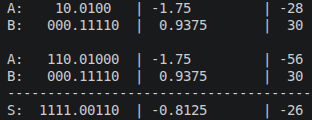
\includegraphics[width=0.6\textwidth]{Figuras/suma_py.png}
    \caption{Salida del script de suma en Python.}
    \label{fig:suma_py}
\end{figure}

Por otro lado, el resultado del testbench de la suma en Verilog se muestra en la \autoref{fig:suma_sv}. observándose entonces que el resultado de los dos desarrollos concuerdan con el resultado esperado en forma teórica.

\begin{figure}[H]
    \centering
    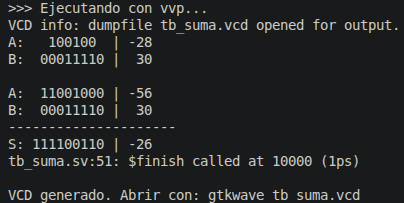
\includegraphics[width=0.6\textwidth]{Figuras/suma_sv.png}
    \caption{Impresión del testbench de suma.}
    \label{fig:suma_sv}
\end{figure}



\subsection{Truncado, Redondeo y Saturación}                        \label{sec_2.3}
En esta sección se aborda la implementación y verificación en \textit{HW} de las técnicas de recorte (truncamiento, redondeo y saturación) para señales en formato de punto fijo. Como paso inicial, se utilizó la librería \texttt{fxpmath} de \textit{Python} para generar un \textit{benchmark} que permita contrastar los resultados de la simulación.

Para el análisis se plantearon los siguientes casos:
\begin{itemize}
    \item Conversión de la señal $x = 5.5625$ del formato $S(10,6)$ al formato $S(7,3)$ aplicando truncamiento y redondeo al más cercano.
    \item Conversión de la señal $y = 8.75$ del formato $S(11,6)$ al formato $S(5,3)$ aplicando \textit{wrap-around} y saturación. Cabe destacar que se modificó el formato original dictado por la consigna para la señal $y$ (de $S(10,6)$ a $S(11,6)$) añadiendo un bit a la parte entera, con el fin de evitar un desbordamiento (\textit{overflow}) en la señal de entrada.
\end{itemize}

En la \autoref{fig:fig_1} se observa la salida de la terminal, detallando los resultados teóricos esperados generados por el script de referencia.
\begin{figure}[H]
    \centering
    
\includegraphics[width=0.6\textwidth]{Figura 1.png}
    \caption{Resultados del benchmark en \textit{Python} y ejecución del entorno.}
    \label{fig:fig_1}
\end{figure}

Por otro lado, dado que se programo tanto un modulo como un testbench en \textit{Verilog} se propone graficar estos cambios utilizando \textit{GTKWave} tal como se muestra en la \autoref{fig:fig_2}. 
\begin{figure}[H]
    \centering
    
\includegraphics[width=0.9\textwidth]{Figura 2.png}
    \caption{Simulación en GTKWave mostrando las señales de entrada y salida en formato hexadecimal.}
    \label{fig:fig_2}
\end{figure}

Al analizar las formas de onda, se corroboran los siguientes resultados:
\begin{itemize}
    \item \underline{Señal $x$}: La entrada asume el valor $059_{h}$ (en hexadecimal) ($5.5625_{10}$ en base decimal). Tras el recorte, tanto el truncamiento (\texttt{x\_trunc}) como el redondeo (\texttt{x\_round}) arrojan el valor \texttt{0B} ($5.5_{10}$).
    
    \item \underline{Señal $y$}: La entrada asume el valor $230_{h}$ (en hexadecimal) ($8.75_{10}$). Al aplicar un recorte directo por \textit{wrap-around}, se pierden los bits más significativos y el valor resultante cae a \texttt{06} ($0.75_{10}$). Por el contrario, al aplicar lógica de saturación, el \textit{HW} detecta el \textit{overflow} positivo y limita la salida al máximo valor representable en el formato $S(5,3)$, que corresponde a \texttt{0F} ($1.875_{10}$).
\end{itemize}

Los resultados obtenidos en la simulación temporal coinciden con total exactitud con el modelo de referencia.



\subsection{CSD — Recodificación}                                   \label{sec_2.4}

La representación \emph{Canonical Signed Digit} (CSD) es un método utilizado en DSP que ofrece una optimización en la cantidad de sumadores cuando se requiere hacer una multiplicación por una constante, en algunos casos. Esto conlleva a disminuir el área y la potencia, pero la constante debe tener varios unos consecutivos para obtener una mejora significativa.

Se realizó la multiplicación de una señal variable y signada con el valor $K = 23$, en binario estándar y en CSD. La conversión de $K$ a CSD se muestra en la \autoref{tab:csd}. De esta forma, se obtiene un coeficiente sin no-ceros consecutivos y se espera que la cantidad de sumas realizadas en una multiplicación pasen de 3 a 2.

\begin{table}[H]
    \centering
    \begin{tabular}{r|cccccc}
         Binario & 0 & 1 & 0 & \color{red}1 & \color{red}1 & \color{red}1 \\
          & 0 & \color{red}1 & \color{red}1 & 0 & 0 & -1 \\
         CSD & 1 & 0 & -1 & 0 & 0 & -1 \\
    \end{tabular}
    \caption{Conversión del valor K a CSD.}
    \label{tab:csd}
\end{table}

Realizando la multiplicación de K por una señal S(4,0) en Python, se obtiene el resultado de la \autoref{fig:csd_py}. Si se observa el código de la multiplicación en la \autoref{fig:csd_sumas_py}, se puede ver que se redujo la cantidad de sumadores como se esperó, ya que se usaron 3 sumas en el caso del binario estándar y 2 sumas en el caso del CSD.

La implementación del módulo en Verilog se realizó con el mismo algoritmo y el testbench arrojó los mismos resultados que el algoritmo de Python. Estos se muestran en la \autoref{fig:csd_sv}. Nuevamente, en el RTL se comprueba la reducción de sumadores, como se muestra en la \autoref{fig:csd_sumas_sv}.

\begin{figure}[H]
    \centering
    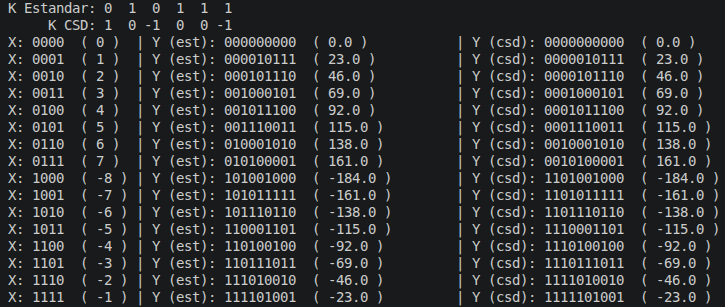
\includegraphics[width=0.9\textwidth]{Figuras/csd_py.png}
    \caption{Resultado impreso de la multiplicación en binario estándar y con CSD en Python.}
    \label{fig:csd_py}
\end{figure}

\begin{figure}[H]
    \centering
    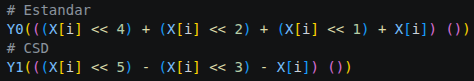
\includegraphics[width=0.7\textwidth]{Figuras/csd_sumas_py.png}
    \caption{Asignación de la multiplicación en Python.}
    \label{fig:csd_sumas_py}
\end{figure}

\begin{figure}[H]
    \centering
    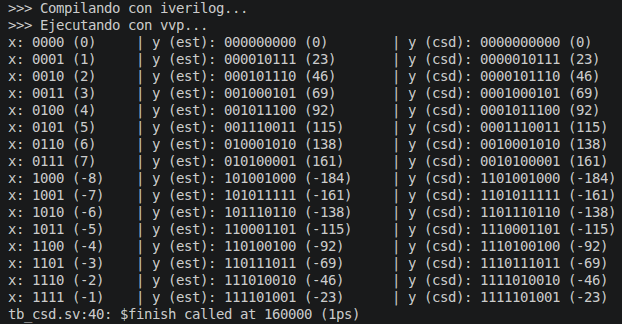
\includegraphics[width=0.9\textwidth]{Figuras/csd_sv.png}
    \caption{Resultado del testbench, en binario estándar y con CSD en Verilog.}
    \label{fig:csd_sv}
\end{figure}

\begin{figure}[H]
    \centering
    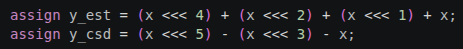
\includegraphics[width=0.7\textwidth]{Figuras/csd_sumas_sv.png}
    \caption{Asignación de la multiplicación en Verilog.}
    \label{fig:csd_sumas_sv}
\end{figure}

\subsection{Booth \texttt{radix-2}}                                 \label{sec_2.5}
En este ejercicio se implementó un multiplicador por \textit{HW} utilizando el algoritmo de \textit{Booth} \texttt{radix-2}. El objetivo consistió en realizar el producto de dos números signados de $4$ bits representados en complemento a $2$: el multiplicando $A = +6$ y el multiplicador $B = -5$. 

Para aplicar el algoritmo, se extendió el multiplicador $B$ agregando un bit virtual $b_{-1} = 0$ en la posición menos significativa, permitiendo evaluar los pares de bits $(b_i, b_{i-1})$ para determinar las sumas y restas de los productos parciales desplazados.

Como paso preliminar, se generó un modelo de referencia en Python utilizando la librería \texttt{fxpmath}, cuyos resultados por consola se detallan en la \autoref{fig:fig_3}.
\begin{figure}[H]
    \centering
    
\includegraphics[width=0.8\textwidth]{Figura 3.png}
    \caption{Resultados del benchmark en \textit{Python} y ejecución de la compilación.}
    \label{fig:fig_3}
\end{figure}

El script de referencia calculó que el producto de dos señales de $4$ bits genera un resultado de $8$ bits. Posteriormente, se simuló el \textit{HW} diseñado en \textit{Verilog} y se visualizaron los resultados temporales mediante \textit{GTKWave}, como se muestra en la \autoref{fig:fig_4}.
\begin{figure}[H]
    \centering
    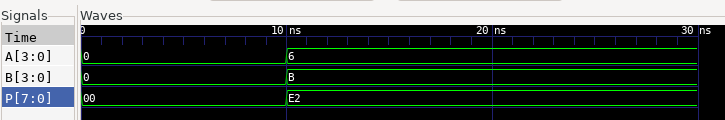
\includegraphics[width=0.9\textwidth]{Figura 4.png}
    \caption{Simulación en GTKWave del multiplicador Booth radix-2.}
    \label{fig:fig_4}
\end{figure}

Al analizar las formas de onda de la \autoref{fig:fig_4}, se verifica la correcta operación del módulo:
\begin{itemize}
    \item \underline{Multiplicando (A):} El valor de entrada es \texttt{6} en hexadecimal, correspondiente a $0110_{2}$ o $+6_{10}$ en complemento a 2.
    \item \underline{Multiplicador (B):} El valor de entrada es \texttt{B} en hexadecimal, correspondiente a $1011_{2}$ o $-5_{10}$ en complemento a 2.
    \item \underline{Producto (P):} La salida obtenida es \texttt{E2} en hexadecimal. Su representación binaria es $11100010_{2}$, lo que equivale exactamente a $-30_{10}$ en complemento a 2.
\end{itemize}

De esta manera, se comprueba que el comportamiento del \textit{HW} diseñado coincide con la verificación teórica $A \cdot B = -30$ establecida en la consigna.



\subsection{RNS — Multiplicación Modular}                           \label{sec_2.6}

El sistema de representación \emph{Residue Number System} (RNS) consiste en representar un número entero por sus residuos respecto a valores coprimos, resultando en varias operaciones más pequeñas en paralelo y sin propagación de carry. Esto puede aumentar el area pero permite un paralelismo muy alto.

Tomando dos ejemplos, se representaron dos valores $X$ e $Y$ en RNS, tomando el conjunto de módulos $\{3,5,7\}$, y luego se realizó el producto en cada módulo. El desarrollo en forma teórica se muestra en el \autoref{tab:rns}.

\begin{table}[H]
    \centering
    \begin{tabular}{l|ccc}
        & Mod. 3 & Mod. 5 & Mod. 7 \\
        $X = 14$ & 2 & 4 & 0 \\
        $Y = 6$ & 0 & 1 & 6 \\
        \hline
        $P = 84$ & 0 & 4 & 0 \\
    \end{tabular}
    \caption{Multiplicación modular entre X e Y.}
    \label{tab:rns}
\end{table}

En Python se armó un vector de valores modulares para cada variable y se realizó el producto modular. El resultado se puede ver en la \autoref{fig:rns_py}.

\begin{figure}[H]
    \centering
    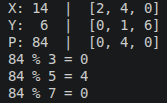
\includegraphics[width=0.2\textwidth]{Figuras/rns_py.png}
    \caption{Resultado del producto modular en Python.}
    \label{fig:rns_py}
\end{figure}

Mientras tanto, en Verilog no se utilizó un arreglo de valores modulares, sino que se usaron 3 variables internas para cada señal, cada una con distinto número de bits para optimizar el área. Para la multiplicación modular, se utilizó el operador ``\%'', que no es sintetizable pero es útil para observar este caso en particular. El resultado puede observarse en la \autoref{fig:rns_sv} y se comprueba el resultado correcto en comparación con el teórico.

\begin{figure}[H]
    \centering
    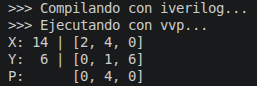
\includegraphics[width=0.4\textwidth]{Figuras/rns_sv.png}
    \caption{Resultado del producto modular en Verilog.}
    \label{fig:rns_sv}
\end{figure}

\section{Conclusiones}                                              \label{sec_3}

Este trabajo presenta la implementación de varias formas de representación y calculo numérico en un DSP, desarrolladas tanto en Python como en Verilog. Se realizó la conversión en formato de punto flotante y punto fijo, en algunos casos sin pérdida de cuantización pero en otros con necesidad de aplicar truncamiento y/o saturación. Se estudiaron pocos casos de suma y producto en punto fijo pero con el objetivo de explorar varios tipos de representación, en este caso el CSD, Booth radix-2 y RNS. En todos los casos, los modelos de Python y Verilog coincidieron perfectamente.

\newpage
\nocite{*}
\printbibliography[heading=bibintoc, title={4. \ Referencias}]
\end{document}